%
% teil3.tex -- Beispiel-File für Teil 3
%
% (c) 2020 Prof Dr Andreas Müller, Hochschule Rapperswil
%
% !TEX root = ../../buch.tex
% !TEX encoding = UTF-8
%
\subsection{Selektion
\label{buch:paper:varalg:subsection:selection}}
\rhead{Selektion}
In diesem Schritt werden Elternpaare ausgewählt, aus denen neue 
Nachkommen erzeugt werden. Die Selektion erfolgt so, dass in der 
Regel nur die Fittesten die Chance erhalten, neue Kinder zu erzeugen. 
Ein wichtiger Punkt ist, dass, obwohl die Fittesten bevorzugt werden, 
auch die weniger Fitten die Möglichkeit haben, Nachkommen zu erzeugen. 
Dadurch wird sichergestellt, dass die Population nicht zu schnell 
konvergiert\footnote{
    Konvergenz bedeutet, dass die Population von Lösungen immer ähnlicher wird
    }
und in einem lokalen Minimum stecken bleibt. Durch die weniger Geeigneten 
wird die Vielfalt der Population erhalten und somit die Chance erhöht, 
dass die Population nicht in einem lokalen Minimum steckenbleibt. Die Abbildung
\ref{fig:selection_of_parents} stellt dies bildlich dar.
\begin{figure}
    \centering
    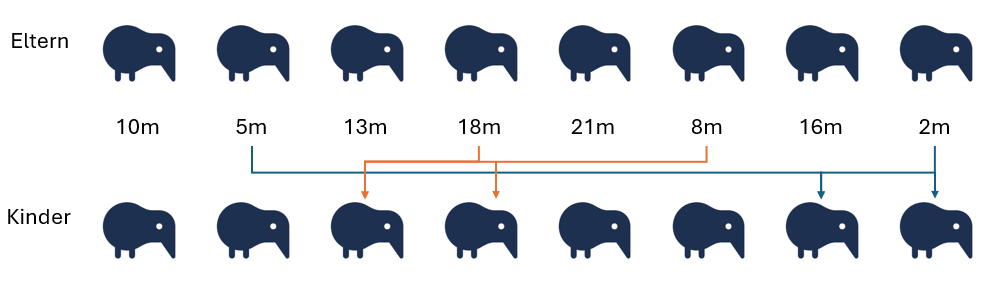
\includegraphics[width=0.8\textwidth]{
        papers/varalg/images/teil3/04OffspringProbability.png
    }
    \caption{
        Mögliche ausgewählte Eltern für Nachkommen, wobei die blaue Linie 
        eine höhere Wahrscheinlichkeit hat als die rote Linie}
    \label{fig:selection_of_parents}
\end{figure}
Für die Selektion gibt es verschiedene Möglichkeiten.
\begin{enumerate}
    \item \textbf{Roulette-Rad-Selektion:} Individuen werden zufällig und
    proportional zu ihrer Fitness ausgewählt. Die Wahrscheinlichkeit wird 
    anhand ihrer Fitness definiert. Kürzere Strecken haben eine höhere Chance, 
    ausgewählt zu werden. Die Wahrscheinlichkeit lässt sich mit der Formel
    \begin{equation}
        P_i
        =
        \frac{f_i}{\sum_{j=1}^{N} f_j}
        \label{buch:paper:varalg:selection:probability_fittest}
    \end{equation}
    berechnen. \(f_i\) ist die Funktion, welche die Fitness des Individuums berechnet.
    Geteilt durch die Totale Fitness. \(P_i\) ist die Wahrscheinlichkeit für das Individuum
    \item \textbf{Rangselektion:} Individuen werden nach ihrer Fitness sortiert und basierend
    auf ihrem Rang ausgewählt. Die Wahrscheinlichkeit wird anhand des Rangs definiert. Die 
    Formel 
    \begin{equation}
        P_i
        =
        \frac{r_i}{\sum_{j=1}^{N} r_j}
        \label{buch:paper:varalg:selection:probability_rating}
    \end{equation}
    ist die gleiche wie oben, verwendet jedoch die Funktion \(r_i\), welche den 
    Rang des Individuums berechnet.
    \item \textbf{Turnierselektion:} Eine Gruppe von Individuen wird zufällig ausgewählt
    und das fitteste Individuum dieser Gruppe wird als Elternteil gewählt.
\end{enumerate}
Es gibt auch die Möglichkeit, ein eigenes Selektionssystem zu entwickeln, 
das ein Ausscheidungsverfahren beinhaltet, aus dem schliesslich ein 
Elternpaar hervorgeht. Das System folgt einem logischen Ablauf, wobei 
die Wahrscheinlichkeit mathematisch berechnet wird.

\subsection{Selektion auf das TSP angepasst
\label{buch:paper:varalg:subsection:selection_tsp}}
\rhead{Selektion TSP}
Für das Traveling Salesman Problem muss die Fitness nach der kürzeste Strecke,
definiert sein. Dass bedeutet, dass die Wahrscheinlichkeit für die Selektion
so umgestellt werden, dass je kürzer die Strecke, desto höher die Wahrscheinlichkeit
ist. Die Formel \ref{buch:paper:varalg:selection:probability_fittest} wird 
dafür angepasst und neu zu
\begin{equation}
    P_i
    =
    \frac{\frac{1}{f_i}}{\sum_{j=1}^{N} \frac{1}{f_j}}
    \label{buch:paper:varalg:selection:probability_fittest_tsp}
\end{equation}
, dabei wird die Fitness mit \(\frac{1}{f_i}\) umgekehrte.
